\documentclass[a4paper,twoside]{article}

\usepackage{epsfig}
\usepackage{subfigure}
\usepackage{calc}
\usepackage{amssymb}
\usepackage{amstext}
\usepackage{amsmath}
\usepackage{amsthm}
\usepackage{multicol}
\usepackage{pslatex}
\usepackage{apalike}
\usepackage{SciTePress}
\usepackage[small]{caption}

\subfigtopskip=0pt
\subfigcapskip=0pt
\subfigbottomskip=0pt

\begin{document}
	
	\title{\uppercase{Entwicklung eines Dateitransfer-Klienten mittels Methoden der modellgetriebenen Software-entwicklung}}
	
	\author{\authorname{Mario Kaulmann\sup{1}, Naoufel Frioui\sup{1} and Carole Noutchegueme\sup{1}}
		\affiliation{\sup{1}Fachbereich Informatik und Medien, Technische Hochschule Brandenburg, Magdeburger Stra\ss{}e 50, Brandenburg an der Havel, Deutschland}
	}
	
	\keywords{MDSD, modellgetriebene Software-Entwicklung, md2, Dateitransfer, REST, Android}
	
	\abstract{Bei modelgetriebener Software-Entwicklung wird versucht Code zu generieren, ohne tiefgehende Programmierkenntnisse vorauszusetzen. In dieser Arbeit wurde mit $\text{MD}^2$ versucht eine Android-App zu erstellen, mit der man Dateien \"uber einen REST-Service versenden kann. Au\ss{}erdem soll man sich bei der App \"uber den REST-Service anmelden und registrieren k\"onnen. Dabei wurden Grenzen von $\text{MD}^2$ ermittelt und ein eigenes speziell auf das Projekt angepasstest Tool (Feature Provider) wurde erstellt, damit fehlende Eigenschaften der App automatisch generiert werden k\"onnen. Zur besseren Umsetzung des Feature Providers wurde die App auf klassische Weise programmiert, um so Kentnisse dar\"uber zu erlangen, wie der Feature Provider arbeiten muss.}
	
	\onecolumn \maketitle \normalsize \vfill
	\section{\uppercase{Einleitung}}
	\label{sec:introduction}
	
	\subsection{Motivation}
	Modellgetriebene Software-Entwicklung (MDSD) soll dazu dienen das Entwickeln von Anwendungen so zu vereinfachen, dass Menschen ohne Programmierkenntnisse, Anwendungen erstellen k\"onnen, die f\"ur einen speziellen Anwendungsbereich eingesetzt werden k\"onnen.\\
	Das Entwickeln einer Smartphone-App ist eine komplexe Aufgabe. Wenn diese App mit einem Server kommunizieren soll, dann wird die Komplexit\"at dieser Aufgabe noch erh\"oht.\\
	Um trotzdem Ergebnisse erzielen zu k\"onnen gibt es bereits Ans\"atze, mit deren Hilfe man durch Beschreibungen des Problems Code erzeugen kann, durch den eine lauff\"ahige Anwendung entsteht. 
	
	\subsection{Ziel}
	Das Ziel besteht darin eine Android-App mit Hilfe von Methoden der MDSD zu erstellen. Die App soll \"uber eine REST-Schnittstelle Dateien auf einen Server laden k\"onnen und Dateien von diesem Server runterladen k\"onnen. Damit verschiedene Nutzer den Dateitransfer-Dienst nutzen k\"onnen, soll auch eine Funktion bereitgestellt werden, die es erm\"oglicht, dass Nutzer sich registrieren, anmelden und abmelden k\"onnen. Diese Funktionen werden von dem Server bereitgestellt und sind auch \"uber eine REST-Schnittstelle nutzbar.\\
	Bei der Umsetzung dieses Vorhabens wird herausgestellt, was mit den zum Zeitpunkt der Arbeit verf\"ugbaren Mitteln m\"oglich ist und welche Grenzen es noch gibt.
	
	\subsection{Aufgabenstellung}
	Zum Vergleichen des Ergebnisses, das mit Methoden der MDSD erstellt wird, wird vorher ein Prototyp erstellt, der den vollen Funktionsumfang bietet und auf klassische Weise programmiert wird.\\
	Im ersten Schritt der Entwicklung werden Mittel zur modellgetriebenen Entwicklung eines Android-Klienten ausgesucht. Im zweiten Schritt wird versucht den Prototyp des Klienten zu entwickeln. Dabei wird der erzeugte Code anschlie\ss{}end in Android Studio ge\"offnet und kompiliert. Anschlie\ss{}end wird die App getestet und mit der klassisch programmierten App verglichen, um die aktuellen Grenzen aufzuzeigen und herauszufinden, ob der Prototyp die Anforderungen erf\"ullt.\\
	Um den Funktionsumfang erf\"ullen zu k\"onnen werden einige Teile bei der MDSD-App mit selbstgeschriebenen Code erg\"anzt.
	
	\subsection{Abgrenzung}
	In dieser Arbeit soll nur ein Android-Klient erstellt werden, der mit einem Server \"uber eine REST-Schnittstelle kommuniziert. Es ist nicht Bestandteil dieser Arbeit eine Server-Anwendung zu erstellen, die die REST-Schnittstelle zur Verf\"ugung stellt.\\
	Das Produkt dieser Arbeit ist ein Prototyp, der durch verschiedene MDSD-Methoden erstellt wird. Der Anteil des selber geschriebenen Codes wird dabei versucht m\"oglichst klein zu halten.
	
	\subsection{Ergebnis}
	Am Ende der Arbeit gibt es eine App, die mit $\text{MD}^2$ generiert wurde und mit einem selbstgeschriebenen Feature Provider verbessert wurde. Die Vergleichs-App, die auf klassische Weise programmiert wurde, hat allerdings mehr Funktionen und bietet sch\"onere Views. Durch das Erstellen des Feature Providers konnten verschiedene M\"oglichkeiten Quellcode f\"ur Android Apps automatisiert zu ver\"andern und neu zu generieren ausprobiert werden.
	
	\section{\uppercase{Vorgehen}}
	
	\subsection{App-Entwicklung}
	
	\noindent Parallel zu diesem Projekt befindet sich auch der Server, der verwendet werden soll in der Entwicklung. Zum Testen des Servers wurde eine Web\-ober\-fl\"ache bereitgestellt.\footnote{http://34.238.158.85/MDSD-2017\_2018/doc/swagger-ui-master/dist/index.html} \\
	Um die Umsetzung eines Zugriffs auf einen REST-Service in Android zu testen, wurde ein Prototyp auf klassische Weise programmiert. Das bedeutet, dass der Code in Android Studio ausgehend von einem leeren Projekt entwickelt wird. Dabei werden einerseits Erkenntnisse generiert, wie die Verbindung mit dem REST-Server funktioniert und allgemein, wie die App in Android umgesetzt wird, sodass man sieht, was in welche Dateien geschrieben werden muss und wie diese strukturiert sind.\\
	Au\ss{}erdem wurde die App auch mit Hilfe von $\text{MD}^2$ umgesetzt. Dabei sieht man die Grenzen die bei $\text{MD}^2$ noch bestehen. Den Code der von $\text{MD}^2$ generiert wurde kann man dann analysieren und mit dem auf klassische Weise erzeugten Code vergleichen. Da bei der Erzeugung des $\text{MD}^2$-Codes ebenfalls Muster entstehen, die im Rahmen der in Android g\"ultigen Strukturen bestehen, kann man diese nutzen, um ein weiteres Programm zu erzeugen, dass die fehlenden Elemente automatisch erzeugt.\\
	Die Abbildung \ref{fig:Arbeitsschritte} zeigt das Vorgehen bei der Entwicklung der $\text{MD}^2$-App.
	
	\begin{figure}[!h]
		%\vspace{-0.2cm}
		\centering
		{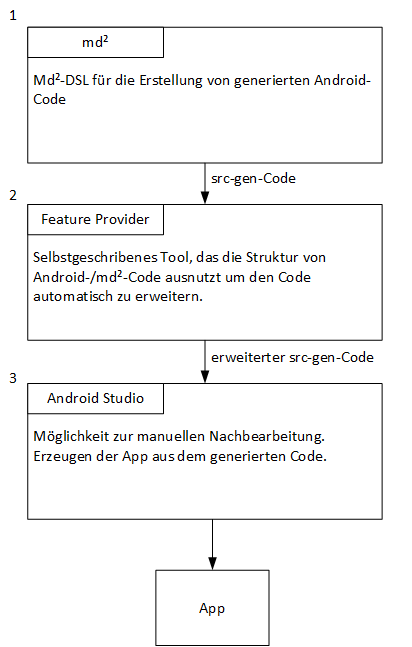
\epsfig{file = Abbildungen/Arbeitsschritte.png, width = 5.5cm}}
		\caption{Es werden die einzelnen Arbeitsschritte dargestellt. Die Zahlen geben die Reihenfolge der Schritte an. An den Pfeilen steht die Ausgabe des Vorg\"angerschritts, die als Eingabe des n\"achsten Schritts dient.}
		\label{fig:Arbeitsschritte}
	\end{figure}
	
	\noindent Der Code, der von $\text{MD}^2$ erzeugt wird, wird in einen Ordner mit dem Namen "src-gen" gespeichert. Auf diesem Code arbeitet der Feature Provider weiter. Das Ergebnis des Feature Providers wird in dem gleichen Ordner gespeichert. Nachdem der Code erweitert wurde kann er mit Android Studio ge\"offnet werden. Bei Bedarf k\"onnen manuelle Ver\"anderungen an dem Code vorgenommen werden. In Android Studio kann die App dann kompiliert und getestet werden.
	
	\subsection{Feature Provider-Entwicklung}
	Bei der Entwicklung des Feature Providers werden die Erkenntnisse der klassischen Programmierung ausgenutzt. Dabei werden allgemein g\"ultige Konzepte benutzt, sowie das Wechseln einer Activity mit Hilfe eines Intents. F\"ur die Umsetzung der Kommunikation mit einem REST-Service gibt es verschiedene Bibliotheken. Der Feature Provider benutzt ausschlie\ss{}lich die Bibliotheken, die bei der klassisch programmierten App benutzt wurden.\\
	Zuerst wurde die Benutzeroberfl\"ache entwicklet, die es erm\"oglicht die entsprechenden Einstellungen auszuw\"ahlen. Besonders wichtig ist, die Auswahl des "src-gen"-Ordners, da der Absolute Pfad zu diesem Ordner auf jedem Ger\"at anders ist.\\
	Danach wurde die Funktionalit\"at des Erzeugens der Features implementiert.\\
	Zur Entwicklung der Funktionalit\"at des Feature Providers wurde in den von $\text{MD}^2$ erzeugten Code geschaut an welcher Stelle zus\"atzlicher Code eingef\"ugt werden muss, oder wo der Code durch anderen ersetzt werden muss. In der klassischen App wurde der Code gepr\"uft, wie die Funktionalit\"at umgesetzt wurde. Bei der Erstellung des Feature Providers wurden dann einige Klassen direkt \"ubernommen mit einigen Ver\"anderungen. Nach der Erzeugung einer neuen Funktion des Feature Providers wurden die in Abbildung \ref{fig:Arbeitsschritte} dargestellten Arbeitsschritte durchgef\"uhrt um zu testen, ob die App dann noch funktioniert und um zu sehen, dass das gewollte Feature hinzugef\"ugt wurde.
	
	\section{\uppercase{Entwicklung}}
	\subsection{Schnittstellen}
	Hier werden die Schnittstellen beschrieben, die mithilfe vom REST-Service vom Server zur Verf\"ugung stehen. Diese basieren auf Standard-HTTP-Operationen.
	\begin{enumerate}
		\item Nutzeroperationen
		\begin{itemize}
			\item Erstellung eines Nutzers (Post)\\
			Hier ist die Erstellung von einem Nutzer m\"oglich. Nur registrierte Nutzer k\"onnen die App benutzen. Daf\"ur braucht man die Parameter: 
			\begin{itemize}
				\item username 
				\item password
			\end{itemize}
			Antwort 200: Die Operation war erfolgreich. Die Antwort enth\"alt die folgenden Werte:
			\begin{itemize}
				\item id (ID des home-Ordners)
				\item home
				\begin{itemize}
					\item subfolders (id, name)
					\item files (id, name)
				\end{itemize}
			\end{itemize}
			
			Antwort 400: Schlechte Anfrage, falls der Nutzer ung\"ultige oder schon vorhandene Parameter eintr\"agt (Passwort zu kurz oder Nutzername zu kurz)
			
			\item Nutzer im System einloggen (Post) \\
			Hier ist das Einloggen von einem Nutzer im System m\"oglich. Diese Funktionnalit\"at ist nur m\"oglich, wenn der Nutzer schon registriert ist. Daf\"ur braucht man: 
			\begin{itemize}
				\item username 
				\item password
			\end{itemize}
			Antwort 200: Die Operation war erfolgreich. Die Dateien, die zur\"uck geschickt sind, sind:
			\begin{itemize}
				\item token
				\item id (ID des home-Ordners)
				\item home
				\begin{itemize}
					\item subfolders (id, name)
					\item files (id, name)
				\end{itemize}
			\end{itemize}
			Antwort 400: Schlechte Anfrage, falls der Nutzer ung\"ultige Parameter eintr\"agt. (Nutzer nicht im System)
			\item Delete (Meldet die aktuelle angemeldete Benutzersitzung ab)
			Hier ist die Abmeldung von der Sitzung m\"oglich. Daf\"ur braucht man den Token vom Nutzer. \\
			Antwort 200: Die Operation war erfolgreich. 
			Antwort 400: Schlechte Anfrage, der angegebene Token ist nicht vergeben.
		\end{itemize}
		
		\item Dateioperationen
		\begin{itemize}
			\item Hochladen von Dateien (Post)
			Hier ist das Hochladen von einer Datei m\"oglich. Daf\"ur braucht man: 
			\begin{itemize}
				\item token
				\item folderId 
				\item file
			\end{itemize}
			Antwort 200: Die Operation war erfolgreich. Die Antwort enth\"alt folgende Parameter:
			\begin{itemize}
				\item id (id des Ordners)
				\item subfolders (id, name)
				\item files (id, name)
			\end{itemize}
			Antwort 400: Schlechte Anfrage, Im Fall die Gr\"o{\ss}e der Datei gr\"o{\ss}er als 30Mb ist. \\
			Antwort 403: Verboten (ung\"ultiger Token) \\
			Antwort 404: Ordner nicht gefunden
			\item Herunterladen von Dateien (Get)
			Hier ist das Herunterladen von einer Datei m\"oglich. Daf\"ur braucht man:
			\begin{itemize}
				\item token
				\item folderId (Id vom \"ubergeordneten Ordner)
				\item fileId (Id von der Datei)
			\end{itemize}
			Antwort 200: Die Operation war erfolgreich. Die Antwort hat folgende Parameter:
			\begin{itemize}
				\item id (id des Ordners)
				\item subfolders (id, name)
				\item files (id, name)
			\end{itemize}
			Antwort 403: Verboten (ung\"ultiger Token) \\
			Antwort 404: Datei / Ordner nicht gefunden
			\item Bearbeitung vom Dateiname (Put)
			Hier ist die Bearbeitung von einer Datei m\"oglich. Daf\"ur braucht man:
			\begin{itemize}
				\item token
				\item folderId (Id vom \"ubergeordneten Ordner)
				\item fileId (Id von der Datei)
				\item name (Der Name von der Datei) 
			\end{itemize}
			
			Antwort 200: Die Operation war erfolgreich. Die Antwort hat folgende Parameter:
			\begin{itemize}
				\item id (id des Ordners)
				\item subfolders (id, name)
				\item files (id, name)
			\end{itemize}
			Antwort 400: Schlechte Anfrage \\
			Antwort 403: Verboten \\
			Antwort 404: Nicht gefunden
			\item L\"oschen von einer Datei (Delete)
			Hier ist das L\"oschen von einer Datei m\"oglich. Daf\"ur braucht man: 
			\begin{itemize}
				\item token
				\item folderId (Id vom \"ubergeordneten Ordner)
				\item fileID (Id von der Datei)
			\end{itemize}
			Antwort 200: Die Operation war erfolgreich. 
			Antwort 403: Verboten (ung\"ultige Token) \\
			Antwort 404: Datei / Ordner nicht gefunden
		\end{itemize}
		
		\item Verzeichnisoperationen
		\begin{itemize}
			\item Herunterladen von einem Ordner (Get)
			Hier ist das herunterladen von einem Ordner m\"oglich. Daf\"ur braucht man: 
			\begin{itemize}
				\item token
				\item folderId (Id vom Ordner) 
			\end{itemize}
			Antwort 200: Die Operation war erfolgreich. Die Antwort hat folgende Parameter:
			\begin{itemize}
				\item id (id des Ordners)
				\item subfolders (id, name)
				\item files (id, name)
			\end{itemize}
			Antwort 403: Verboten \\
			Antwort 404: Nicht gefunden
			\item Erstellen eines Ordners (Post) \\
			Hier ist das Erstellen von einem Ordner m\"oglich. Daf\"ur braucht man:
			\begin{itemize}
				\item token
				\item folderId (id des \"ubergeordneten Ordners)
				\item folder (Name des neuen Ordners)
			\end{itemize}
			Antwort 200: Die Operation war erfolgreich. Die Antwort hat folgende Parameter:
			\begin{itemize}
				\item id (id des Ordners)
				\item subfolders (id, name)
				\item files (id, name)
			\end{itemize}
			Antwort 400: Schlechte Anfrage, Im Fall die Gr\"o{\ss}e der Datei gr\"o{\ss}er als 30Mb ist. \\
			Antwort 403: Verboten \\
			Antwort 404: Nicht gefunden
			\item Bearbeitung von einem Ordner (Put) \\
			Hier ist die Bearbeitung von einem Ordner m\"oglich. Daf\"ur braucht man: 
			\begin{itemize}
				\item token
				\item folderId (Id vom \"ubergeordneten Ordner) 
				\item folder (ein neuer Name) 
			\end{itemize}
			Antwort 200: Die Operation war erfolgreich. Die Antwort hat folgende Parameter:
			\begin{itemize}
				\item id (id des Ordners)
				\item subfolders (id, name)
				\item files (id, name)
			\end{itemize}
			Antwort 400: Schlechte Anfrage \\
			Antwort 403: Verboten \\
			Antwort 404: Nicht gefunden
			\item Delete \\
			Hier ist das L\"oschen von einem Ordner m\"oglich. Daf\"ur braucht man: 
			\begin{itemize}
				\item token
				\item folderId (Id vom \"ubergeordneten Ordner) 
			\end{itemize}
			Antwort 200: Die Operation war erfolgreich.
			Antwort 403: Verboten \\
			Antwort 404: Nicht gefunden
		\end{itemize}
	\end{enumerate}
	
	\subsection{klassische App}
	
	Die klassische App wurde programmiert, um zu testen, wie man eine Android-App mit einem REST-Service verbindet. Daf\"ur wurden ein paar Bibliotheken ausprobiert. Die App setzt alle Funktionen um, die vorher festgelegt wurden. Diese Funktionen sind:
	\begin{itemize}
		\item Datei-Upload
		\item Datei-Download
		\item Ordner erstellen
		\item Nutzer registrieren
		\item Nutzer anmelden
		\item Foto machen und hochladen
	\end{itemize}
	
	\noindent Die klassische App benutzt die folgenden externen Bibliotheken:
	\begin{itemize}
		\item loopj\footnote{https://github.com/loopj/android-async-http}\\
		stellt einen asynchronen callback-basierten HTTP-Client basierend auf Bibliotheken von Apache zur Verf\"ugung.
		\item okio\footnote{http://square.github.io/okio/1.x/okio/}\\
		erleichtert den Zugriff, Speicherung und die Verarbeitung von Dateien.
		\item EasyPermission\footnote{https://firebaseopensource.com/projects/googlesamples/easypermissions/} \\
		ist eine Wrapper-Bibliothek zur Vereinfachung der grundlegenden Systemberechtigungslogik f\"ur Android.
		\item okhttp\footnote{http://square.github.io/okhttp/} \\
		wird benutzt um schnelle Input- und Output-Operationen durchzuf\"uhren und gr\"o\ss{}enver\"anderbare Puffer zu benutzen.
		\item Retrofit\footnote{http://square.github.io/retrofit/} \\
		wird genutzt, um die Dateitransfers zu erm\"oglichen. Es k\"onnen auch synchrone und asynchrone Anfragen \"uber HTTP gesendet werden.
	\end{itemize}
	
	\section{\uppercase{Werkzeuge zur Entwicklung}}
	
	\subsection{$\text{MD}^2$}
	$\text{MD}^2$-DSL ist eine dom\"anenspezifische Sprache (DSL), die entwickelt wurde um datengetriebene Business-Apps in textueller Form beschreiben zu k\"onnen \cite{DSLMD2_2013}.\\
	$\text{MD}^2$ ist ein akademischer Prototyp, der auch Anwendung in praktischen Projekten findet und dabei auch weiterentwickelt wird \cite{MDCP2015}.\\
	In diesem Projekt wurde die aktuelle Version von $\text{MD}^2$ verwendet, die auf dem git-Repository\footnote{https://github.com/wwu-pi/md2-framework} zur Verf\"ugung stand (Stand: 23.11.2017). Diese steht als Plugin f\"ur Eclipse zur Verf\"ugung.\\
	$\text{MD}^2$ ist nach dem MVC Prinzip aufgebaut und hat dazu Workflow-Elemente, die spezielle Controller-Elemente sind \cite{Handbookmd2}. Durch das erste Workflow-Element wird immer beim Build des Projekts eine "StartActivity" erzeugt, deren View Buttons enth\"alt zum Starten der Programmierten App.\\
	Der Umfang, der in dem Handbuch f\"ur Modellierer versprochen wurde konnte nicht komplett genutzt werden. Au\ss{}erdem gab es Standardfunktionen, wie das Schlie\ss{}en der App, die nicht umgesetzt waren.\\
	Nach jedem Build des Projektes wurde der alte Code komplett ersetzt durch den neu generierten Code. Dadurch wurden auch manuelle Erweiterungen des Codes zerst\"ort. Aus diesem Grund entstand die Idee, ein Tool zu entwickeln, das automatisch die Erweiterungen des Quellcodes wieder hinzuf\"ugt, die die Funktionalit\"at der App erweitert haben.
	
	\subsection{Android Studio}
	In diesem Projekt wird die freie integrierte Entwicklungsumgebung Android Studio zum Testen der $\text{MD}^2$-App verwendet und um den klassisch programmierten Client zu implementieren. Dadurch k\"onnen Tests auf Smartphones und Emulatoren durchgef\"uhrt werden. Dabei wird auch festgestellt, ob der erzeugte Code von Eclipse und den zus\"atzlich installierten Plugins unabh\"angig ist.
	
	\subsection{Feature Provider}
	Der Feature Provider ist ein Tool, das nur f\"ur die in diesem Projekt entwickelten App erzeugt wurde. Es ist ein Prototyp, der bei seiner Entwicklung dazu beitr\"agt, die Probleme bei MDSD zu verstehen. Ein paar Features k\"onnen in Verbindung mit einer $\text{MD}^2$-App allerdings allgemein genutzt werden.\\
	Nachfolgend werden ein paar Beispiele gegeben, wie der Feature Provider arbeitet.\\
	Das Grund-Feature, dass der Feature Provider immer hinzuf\"ugt ist, dass eine App geschlossen wird, wenn man die erste View sieht und auf den Back-Button dr\"uckt. Der Code, der von $\text{MD}^2$ in der "StartActivity" f\"ur die Aktion "onBackPressed" erzuegt wird sieht wie folgt aus.
	
	\begin{small}
		\begin{verbatim}
		public void onBackPressed() {
		// remain on start screen
		}
		\end{verbatim}
	\end{small}
	
	\noindent Hier ist zu erkennen, dass diese Methode keine Funktion enth\"alt. Aus diesem Grund hat es keine Wirkung, wenn man auf den "Back Button" dr\"uckt.\\
	Der Feature Provider \"offnet die Java-Datei dieser Activity und sucht nach dem Methodenkopf der "onBackPressed"-Methode. Der Kommentar wird dann durch den Code zum Schlie\ss{}en der App ersetzt. Dabei entsteht der folgende Code aus \cite{backclose}:
	
	\begin{small}
		\begin{verbatim}
		public void onBackPressed() {
		Intent intent = new Intent(Intent.ACTION_MAIN);
		intent.addCategory(Intent.CATEGORY_HOME);
		intent.setFlags(Intent.FLAG_ACTIVITY_CLEAR_TOP);
		startActivity(intent);
		finish();
		System.exit(0);
		}
		\end{verbatim}
	\end{small}
	
	\noindent F\"ur die Erzeugung einiger Features m\"ussen mehrere Dateien ver\"andert werden. Zum Beispiel bei der Erzeugung der Funktionen zur Kommunikation mit dem REST-Service. Daf\"ur wird eine Bibliothek\footnote{http://loopj.com/android-async-http/} verwendet, die nicht zum Standard von Android geh\"ort. Diese muss dann in die "build.gradle"-Datei im App-Verzeichnis im Abschnitt "dependencies" eingetragen werden. Hier scheint die Reihenfolge der Eintragungen nicht wichtig zu sein, also kann die Eintragung auch am Anfang der Datei erfolgen. Der Feature Provider sucht in der Datei nach der Zeichenkette "dependencies{" und f\"ugt danach die neue Bibliothek hinzu.\\
		Die Erzeugung der Klassen zur Kommunikation mit dem REST-Service erfolgt mit Hilfe von Klassen, die aus der klassischen App kopiert werden. Diese wurden im Vorfeld so ver\"andert, dass sie in das Projekt nur eingef\"ugt werden m\"ussen und anschlie\ss{}end nur noch verwendet werden m\"ussen. Daf\"ur hat der Feature Provider einen Ordner (Quelldateien), in der vollst\"andige nutzbare Klassen abgelegt sind.\\
		Au\ss{}erdem ist es notwendig die Android-Manifest-Datei zu ver\"andern, da man f\"ur die REST-Services die Berechtigung ben\"otigt ins Internet zu gehen.\\
		Wenn eine Ver\"anderung einer Klasse dazu f\"uhrt, dass eine neue Klasse verwendet wird ist es notwendig, dass entsprechende Import-Statements am Anfang der Klasse erg\"anzt werden. Da die Reheihenfolge hier beliebig ist, werden die neuen Importe direkt nach dem Eintrag "package" gemacht.\\
		Die Erweiterung einer View ben\"otigt mindestens Ver\"anderungen einer Activity, einer XML-Datei zu der View und der "ids.xml"-Datei. Die richtige Platzierung ist in der XML-Datei zur View n\"otig, da diese die Position auf der View beeinflusst. In diesem Projekt wurde implementiert, dass zwei ListView-Elemente in der "DateiDownloadActivity" hinzugef\"ugt werden. Die Platzierung in der View kann dabei frei gew\"ahlt werden. Daf\"ur werden die IDs f\"ur die View-Elemente dem Benutzer des Feature Providers gezeigt und dieser kann w\"ahlen, nach welchem Element er die neue ListView einf\"ugen will. Au\ss{}erdem werden die IDs der neu hinzugef\"ugten Elemente in der "ids.xml"-Datei erg\"anzt. In der Activity wird dann die Lebenszyklusmethode "onCreate" so ver\"andert, dass die ListViews den gew\"unschten Inhalt anzeigen.\\
		Zum Einf\"ugen einer Aktion werden die Klassen im Package "md2.testprojekt.md2.controller.action" ver\"andert. Hier liegen die Klassen, die f\"ur die erzeugten Aktionen benutzt werden. Z.B. wenn man einen Wechsel der Views erzeugt hat, der mit Hilfe eines Buttons realisiert wird.
		
		\section{\uppercase{Zusammenfassung und Ausblick}}
		\noindent Das Werkzeug $\text{MD}^2$ hat sich in der verwendeten Version als nicht so m\"achtig erwiesen, wie es gedacht war, weshalb nur ein geringer Anteil der App mit $\text{MD}^2$ umgesetzt werden konnte. Die Entwicklung eines Feature Providers, der auf dem von $\text{MD}^2$ erzeugten Code weiterarbeitet bot eine M\"oglichkeit das Erzeugen von Quellcode selber umzusetzen, auch wenn der Feature Provider ein sehr eingeschr\"anktes Werkzeug ist, das nur bei diesem Projekt eingesetzt werden kann. Die Umsetzung aller gew\"unschten Funktionen konnte nicht f\"ur die App realisiert werden, die mit $\text{MD}^2$ erzeugt wurde. Allerdings gibt es eine klassisch programmierte App, die den vollen Funktionsumfang bietet, die als Grundlage f\"ur \"Uberlegungen zur Erweiterung des Feature Providers dienen kann. Zuk\"unftig k\"onnten noch weitere Funktionen umgesetzt werden, der Feature Provider k\"onnte allgemeiner gemacht werden, sodass er f\"ur beliebige Anwendungen anwendbar ist.\\
		Methoden der MDSD k\"onnen gut eingesetzt werden, um Android Apps zu generieren. Daf\"ur haben Android Apps entsprechende Strukturen, die sich in der Aufteilung der Code-Elemente wiederfinden. Als Beispiel daf\"ur seinen die Lebenszyklusmethoden genannt und die Aufteilung der View und Activity in verschiedenen Dateien.
	
	\bibliographystyle{apalike}
	\small
	\bibliography{example}
\end{document}